\documentclass{beamer}

\beamertemplatenavigationsymbolsempty

\mode<presentation>
{
  \usetheme{default}
}

\usepackage[english]{babel}
\usepackage[latin1]{inputenc}
\usepackage{bussproofs}
\usepackage[retainorgcmds]{IEEEtrantools}

% needs debian package texlive-math-extra
\usepackage{stmaryrd} % for \llbracket, \rrbracket

\usepackage{times}
\usepackage[T1]{fontenc}
% Or whatever. Note that the encoding and the font should match. If T1
% does not look nice, try deleting the line with the fontenc.

\usepackage{tikz}
\usetikzlibrary{positioning}
\usetikzlibrary{calc}
\usetikzlibrary{matrix}
\usetikzlibrary{arrows}

\title
{Domains for Algebraic Data Types with Computation Steps}

\author
{Markus~Klinik}

\institute[Radboud University Nijmegen]
{
  Radboud University Nijmegen
}

\date
{August 2014}


\newcommand{\arr}{\rightarrow}
\newcommand{\Arr}{\Rightarrow}
\newcommand{\semantics}[1]{\llbracket #1 \rrbracket}
\newcommand{\semanticsFd}[1]{\semantics{#1}_{F\delta}}
\newcommand{\oftype}[2]{#1\!:\!#2}

\begin{document}

\begin{frame}
  \titlepage
\end{frame}

\begin{frame}{Fixpoints, Sums, Products: Pick Two}

\begin{itemize}
\item What? CCC + Fixpoints + Sums = $\lightning$
\item Who? Huwig and Poign\'e, 1990
\item Why? Raising awareness
\item How? Let's see ...
\end{itemize}

\end{frame}


\begin{frame}[fragile]

\begin{definition}
A category is \emph{trivial} iff it has one object with one arrow.
\end{definition}

\begin{definition}
A category has the \emph{fixpoint property} iff every endomorphism has a fixpoint:
$f(Yf) = Yf$
\end{definition}

\begin{center}
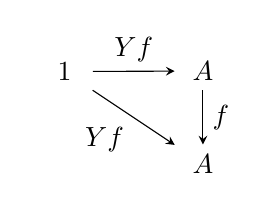
\begin{tikzpicture}
\matrix (m) [matrix of math nodes,row sep=2em,column sep=3em,minimum width=2em]
  {
     1 & A \\
     {} & A \\
  };
  \path[-stealth] (m-1-1) edge node [above] {$Yf$} (m-1-2);
  \path[-stealth] (m-1-1) edge node [below left] {$Yf$} (m-2-2);
  \path[-stealth] (m-1-2) edge node [right] {$f$} (m-2-2);
\end{tikzpicture}
\end{center}

\end{frame}


\end{document}
